The 75 availability issues are collected from 28 subsystems and these subsystems have different numbers of services.
To evaluate the efficiency and scalability of \app, we analyze the execution time of \app~and the two baseline approaches for the 75 availability issues and investigate how the time changes with the size (service number) of the target system.
The results are shown in Figure~\ref{fig:time}.
Note that there may be multiple availability issues collected from the same subsystem and each of them is indicated by a point.

In general, the execution time of \app~is 22.3\% less than that of Microscope and 31.7\% less than that of MonitorRank.
For the subsystems of different sizes \app~uses the least time among the three approaches for most availability issues.
The two curves in Figure~\ref{fig:time} show the changes of the time differences of \app~with the two baseline approaches respectively.
It can be seen that the advantage of \app~is not significant when the number of services is less than 250; when the number of services exceeds 250, the advantage of \app~is getting more and more significant with the increase of service number.
Moreover, the execution time of \app~(also the two baseline approaches) increases linearly with the increase of service number, showing a good scalability.

\begin{figure}[ht]
	\centering
	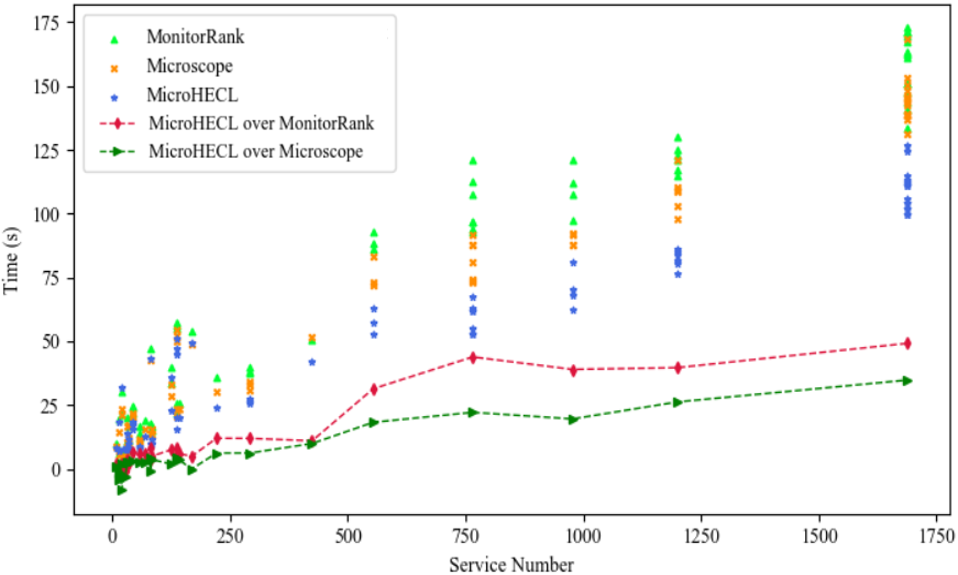
\includegraphics[width=0.5\textwidth]{images/nodes_to_time.png}
	\vspace{-8pt}
	\caption{Detection Time Changes with Num of Nodes}\label{fig:time}
	\vspace{-5pt}
\end{figure}

The advantages of \app~can be explained by its specially designed mechanisms for anomaly propagation analysis.
MonitorRank traverses the service call graph using random walk algorithm and needs to calculate the correlation scores for a large number of the nodes in the graph.
This process is time-consuming when the graph contains many nodes. 
Microscope traverses all the neighboring nodes of an anomalous node, both upstream and downstream.
Moreover, it has no pruning strategy.
In contrast, \app~considers only a single direction (upstream or downstream) for each anomaly type in anomaly propagation chain extension and uses a pruning strategy to eliminate branches that are likely irrelevant to the anomaly propagation.






